\documentclass{beamer}
\usepackage{geometry}
\usepackage[english]{babel}
\usepackage[utf8]{inputenc}
\usepackage{amsmath}
\usepackage{amsfonts}
\usepackage{amssymb}
\usepackage{tikz}
\usetikzlibrary{quotes, angles}
\usepackage{graphicx}

%\usepackage{pgfplots}
%\pgfplotsset{width=10cm,compat=1.9}
%\usepackage{pgfplotstable}

\setlength{\headheight}{26pt}%doesn't seem to fix warning

\usepackage{fancyhdr}
\pagestyle{fancy}
\fancyhf{}

%\rhead{\small{2 January 2019}}
\lhead{\small{BECA / Dr. Huson / Geometry - Unit 7 Analytic Geometry}}

\renewcommand{\headrulewidth}{0pt}

\title{10th Grade Geometry - Unit 6: Similarity}
\subtitle{Bronx Early College Academy}
\author{Christopher J. Huson PhD}
\date{29 January 2019}

\begin{document}
\frame{\titlepage}
\section[Outline]{}
\frame{\tableofcontents}


\section{Seating Chart 10.1}
  \frame
  {
    \frametitle{Seating Chart 10.1}
    \framesubtitle{How do we work as a team?}

    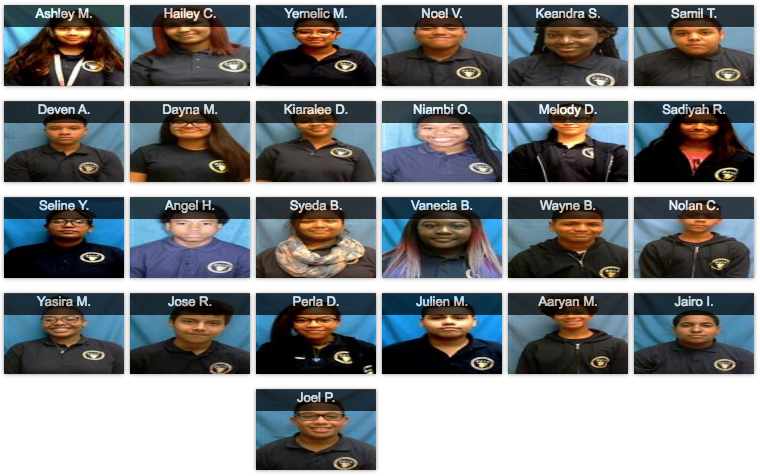
\includegraphics[width=1.05\textwidth]{seating-10A.png}
  }

\section{Seating Chart 10.2}
  \frame
  {
    \frametitle{Seating Chart 10.2}
    \framesubtitle{How do we work as a team?}

    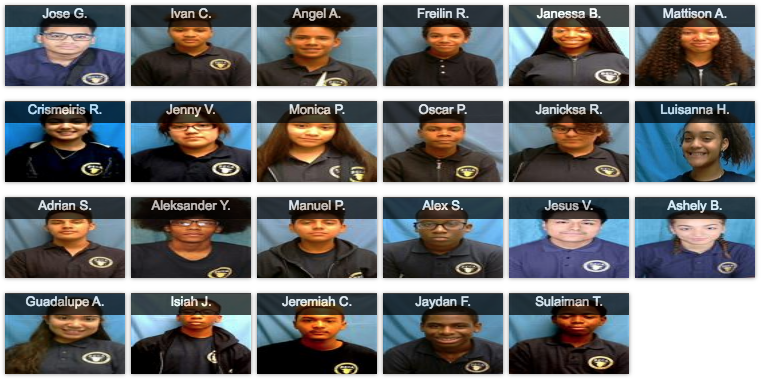
\includegraphics[width=1.05\textwidth]{seating-10B.png}
  }

\section{7.1 Laptops - Geogebra. Tuesday 28 January}
  \frame
  {
    \frametitle{GQ: How do we model with digital tools?}
    \framesubtitle{CCSS: HSG.CO.D.12 Congruence, geometric constructions \hspace{\stretch{1}} \alert{7.1 Tuesday 18 January}}

    \begin{block}{Do Now: Regents review and reflection}
      \begin{itemize}
        \item Results: 10 passing scores, 4 college ready
        \item Top score 75; average 53
        \item 70\% earned free response points
      \end{itemize}
    \end{block}
    GeoGebra Geometry App\\
    Enter \alert{N7BHK} for 10.1 or \alert{P9PNZ} for 10.2\\
    Set up account using your real name.\\
    Beginner Tutorials with Lesson Ideas\\
    Author: Tim Brzezinski\\[0.5cm]
    Homework: Complete Geogebra
  }

\section{7.2 Linear equations. Wednesday 30 January}
  \frame
  {
    \frametitle{GQ: How do we use functions and equations to represent objects on the coordinate plane?}
    \framesubtitle{CCSS: HSG.CO.D.12 Congruence, geometric constructions \hspace{\stretch{1}} \alert{7.2 Wednesday 30 January}}

    \begin{block}{Do Now: Handout}
      \begin{enumerate}
        \item Dilation, plotting equations
      \end{enumerate}
    \end{block}
    Function notation, slope-intercept, standard, \& point slope forms of linear equations\\[0.5cm]
    Homework: Handout review of linear equations and functions
  }

\section{7.3 Linear equations. Thursday 31 January (cold day)}
  \frame
  {
    \frametitle{GQ: How do we use functions and equations to represent objects on the coordinate plane?}
    \framesubtitle{CCSS: HSG.CO.D.12 Congruence, geometric constructions \hspace{\stretch{1}} \alert{7.3 Thursday 31 January}}

    \begin{block}{Do Now: Handout}
      \begin{enumerate}
        \item Translation, plotting equations
      \end{enumerate}
    \end{block}
    Function notation, slope-intercept, standard, \& point slope forms of linear equations\\[0.5cm]
    Homework: Handout review of linear equations and functions
  }

\section{7.4 Slope applications in proof. Friday 1 February}
  \frame
  {
    \frametitle{GQ: How do we use slope in geometric proof?}
    \framesubtitle{CCSS: HSG.CO.D.12 Congruence, geometric constructions \hspace{\stretch{1}} \alert{7.4 Friday 1 February}}

    \begin{block}{Do Now: Handout}
      \begin{enumerate}
        \item Translating segments, plotting equations, perpendicular proof
      \end{enumerate}
    \end{block}
    Applying slope to prove parallel or perpendicular relationships\\[0.5cm]
    Homework: Handout review of linear \& quadratic equations and functions
  }

  \section{7.5 Function translation. Monday 4 February}
    \frame
    {
      \frametitle{GQ: How do we apply translations to functions?}
      \framesubtitle{CCSS: HSG.CO.D.12 Congruence, geometric constructions \hspace{\stretch{1}} \alert{7.5 Monday 4 February}}

      \begin{block}{Do Now: Handout}
        \begin{enumerate}
          \item Translating segments, plotting equations, perpendicular proof
        \end{enumerate}
      \end{block}
      Translating parabolas, vertex form\\[0.5cm]
      Homework: Pretest for review Wednesday. \alert{Test Thursday}
    }




\end{document}
